\documentclass[../main.tex]{subfiles}

\begin{document}

\begin{boxnaslovi}
\section{Imperativna paradigma}
\end{boxnaslovi}
Imperativna paradigma je prvonastala programska paradigma. Nastala je pod uticajem Fon Nojmanove arhitekture računara (tj. ova arhitektura nameće ovaj stil programiranja, prilagođen mašini, a ne čoveku). U rešavanju problema prednost se daje algoritmima pa se imperativno programiranje naziva i {\it Algoritamski orijentisano programiranje}. Podaci i algoritmi postoje nezavisno.
$$ Podaci + Algoritmi = Programi$$
Kao što se u govornom jeziku zapovedni način ({\it imperativ}) koristi za  izražavanje naredbi, tako se imperativni programi mogu posmatrati kao niz naredbi koje računar treba da izvrši. Pored naredbi, ključan je i redosled izvršavanja naredbi -- procedura. Imperativna paradigma i proceduralna paradigma se često koriste kao sinonimi. Imperativno programiranje karakteriše izračunavanje u terminima naredbi koje menjaju {\it stanje }programa.
\\
{\bf Stanje programa} čine sve sačuvane informacije, u datom trenutku vremena, kojima program ima pristup (preko memorije). Izvršavanjem programa generiše se niz stanja. Prelaz iz jednog stanja u sledeće je određen komandama koje se izvršavaju. Svaki imperativni jezik obezbeđuje raznovrsne komande za modifikaciju stanja (manipulisanje) memorije. 
\\
Osnovna komanda za modifikaciju stanja memorije je {\bf naredba dodele}. Ona vrši povezivanje imena i neke vrednosti, odnosno upisivanje konkretne binarne reči na odgovarajuću memorijsku lokaciju. Analogija između memorijskih i (proceduralno) jezičkih elemenata:\\
\begin{tabularx}{\textwidth/3*2}{XXXX}
memorija & binarna reč& mem. registar & adresa\\
\hline
jezik & vrednost& promenljiva& ime
\end{tabularx}
\\
Deklaracijom promenljive u proceduralnom jeziku određuje se veličina memorijskog prostora za zapis promenljive. Na primer:
\begin{center}
\begin{tabular}{ll}
\texttt{Pascal:} & \texttt{var name : Type;} \\
\texttt{C:} & \texttt{type name;} 
\end{tabular}
\end{center}
\pagebreak
Promenljiva se povezuje sa nekom vrednošću preko izraza, što se različito opisuje u različitim jezicima. Na primer:
\begin{center}
\begin{tabular}{ll}
\texttt{Pascal:} & \texttt{V := E} \\
 \texttt{C:} & \texttt{V = E}  \\
\texttt{APL:} & \texttt{V <-- E} 
\end{tabular}
\end{center}

Redosled povezivanja imena i vrednosti (dodeljivanje) utiče na vrednosti izračunavanja:
\begin{Verbatim}
a = 5; b = 3; c = 7;
b = a+1;
c = a+b;	/* Redosled izvrsavanja ovih naredbi je bitan! */
\end{Verbatim}

Bitan je i redosled povezivanja (asocijativnost, prioriteti).
\begin{Verbatim}
b = a + b * c / 2;
\end{Verbatim}

{\bf Kontrola toka} se ostvaruje kroz različite instrukcije i apstrakcije. Najveći broj konstrukcija u imperativnim jezicima je odraz hardverske implementacije. Imperativna paradigma prolazi kroz različite faze razvoja, a svaku fazu karakteriše viši nivo apstrakcije u odnostu na arhitekturu računara, i udaljavanje od asemblerskog jezika. Neki autori svaku fazu imperativne paradigme izdvajaju u posebnu paradigmu, a neki ih tretiraju kao potparadigme imperativne paradigme.
\begin{itemize}
\item Operaciona (pod)paradigma
\item Strukturna (pod)paradigma
\item Proceduralna (pod)paradigma
\item Modularna (pod)paradigma
\end{itemize}

\subsection{Operaciona paradigma}

\begin{tabularx}{\textwidth}{XXXXX}
\texttt{FORTRAN} & \texttt{ALGOL} & \texttt{COBOL} & \texttt{BASIC} & \texttt{\ldots}
\end{tabularx}

Prva faza programiranja. Programiranje je zasnovano na dosetkama, trikovima, naziva se i {\it trik programiranje}. Programi su pisani bez opštih pravila, korišćene su specifičnosti u radu računara, trikovi za uštedu memorije, pisanje samomodifikujućh programa. Dolazi do ogromne produkcije softvera krajem 60-ih godina prošlog veka. 
\\
Kontrola toka se sastoji od minimalnog skupa komandi (koji je često korišćen):
\begin{Verbatim}
komanda ::=
        identifikator = izraz |                   (naredba dodele)
        komanda; komanda |                         (sekvenca)
        labela : komanda |                        (obelezavanje)
        GOTO labela |                             (naredba skoka)
        IF (log_izraz) [THEN] GOTO labela         (selekcija)
\end{Verbatim}

Ove upravljačke strukture su nastale kao odraz (analogoni) struktura u programu na mašinskom jeziku. Prema Fon Nojmanovom konceptu računara, instrukcije slede jedna za drugom (sekvenca naredbi u imperativnom jeziku), a redosled se može promeniti korišćenjem GOTO (Jump) naredbe. U imperativnim jezicima javljaju se 2 oblika GOTO naredbe (u IF naredbi i bez IF naredbe). Korišćenje prethodnih naredbi dovodi do pisanja nepreglednih programa, teških za modifikaciju ({\it ``Špageti-programi''}). To je posledica prilagođavanja jezika mašini, a ne čoveku.
\begin{multicols}{2}
\begin{boxprimer}
Špageti programiranje u C-u
\begin{Verbatim}
#include <stdio.h>

main(){
     float x, y;
     int n;
     n = 1;
    l20: scanf(''%f'', &x);
         y=x;
         if(x<0) goto 130;
         y=-x;
    l30: printf(''y = %f\n'', y);
         n=n+1;
         if (n!=5) goto 120;
}
\end{Verbatim}
\end{boxprimer}

\begin{boxprimer}
Špageti programiranje u Pascal-u
\begin{Verbatim}
program idina;
     label 20, 30;
     var x,y:real;
         n:integer;
begin
    n:=1;
20: readln(x);
    y:=x;
    if x<0 then goto 30;
    y:=-x;
30: writeln(y);
    n:=n+1;
    if n<>5 then goto 20
end.
\end{Verbatim}
\end{boxprimer}

\begin{boxprimer}
Špageti programiranje u C-u
\begin{Verbatim}
main() {
     int i,n;
     float h, x0, x, y;
     printf ("Unsete h, x0 i n\n");
     scanf("%f%f%d",&h,&x0,&n);
     if (n<0) goto komentar;
     printf("Pocetak \n");
     i=0;
poc: x=x0+i*h;
     y=x*x;
     printf("x=%f, y=%f\n", x, y);
     if(i<n) goto uvecanje;
     return 0;
uvecanje: i=i+1; goto poc;
komentar: printf("Nekorektno zadato n\n");
}
\end{Verbatim}
\end{boxprimer}

\begin{boxprimer}
Špageti programiranje u Pascal-u
\begin{Verbatim}
program sagoto;
     label poc, kraj;
     var i,n: integer;
         h, x0, x, y: real;
begin
     writeln (’Unsete h, x0 i n’);
     readln (h, x0, n);
     writeln (’Pocetak’);
     i:=0;
poc: x:=x0+i*h;
     y:=x*x;
     writeln(’x = ’, x, ’ y = ’, y);
     if(i>=n) then goto kraj;
     i:=i+1;
     goto poc;
kraj:
    end.
\end{Verbatim}
\end{boxprimer}

\begin{boxprimer}
Špageti programiranje \\
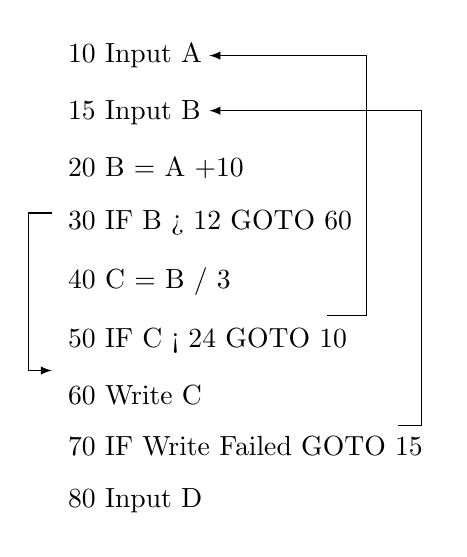
\begin{tikzpicture}[-latex, node distance=0.5mm]
%https://tex.stackexchange.com/questions/66762/tikz-pgf-align-two-text-nodes-to-the-left
\node[right,inner sep=2mm,minimum height=0.6cm] (a) at (1.0, 2.0) {10 Input A};
\node[below right,inner sep=2mm,minimum height=0.6cm] (b) at (a.south west) {15 Input B};
\node[below right,inner sep=2mm,minimum height=0.6cm] (c) at (b.south west) {20 B = A +10};
\node[below right,inner sep=2mm,minimum height=0.6cm] (d) at (c.south west) {30 IF B > 12 GOTO 60};
\node[below right,inner sep=2mm,minimum height=0.6cm] (e) at (d.south west) {40 C = B / 3};
\node[below right,inner sep=2mm,minimum height=0.6cm] (f) at (e.south west) {50 IF C < 24 GOTO 10};
\node[below right,inner sep=2mm,minimum height=0.6cm] (g) at (f.south west) {60 Write C};
\node[below right,inner sep=2mm,minimum height=0.6cm] (h) at (g.south west) {70 IF Write Failed GOTO 15};
\node[below right,inner sep=2mm,minimum height=0.6cm] (i) at (h.south west) {80 Input D};

\draw[-latex] (1,0) -- (0.7,0) -- (0.7,-2) -- (1,-2) ;
\draw[-latex] (4.5, -1.3) -- (5,-1.3 ) -- (5,2) -- (3,2);
\draw[-latex] (5.4, -2.7) -- (5.7, -2.7) -- (5.7, 1.3) -- (3,1.3);
\end{tikzpicture}
\end{boxprimer}

Problemi
\begin{itemize}
\item Teška čitljivost programa i održavanje programa.
\item Kreirani softver je nepogodan za izmene i prilagođavanje novim situacijama.
\item Softverska kriza 1970-ih, zbog loše prakse programiranja softver nije mogao da dostigne mogućnosti hardvera.
\item Uzrok: nekontrolisana upotreba GOTO-naredbe.
\item Rešenje: strukturno programiranje -- disciplinovan pristupu programiranju, bez nekontrolisanih skokova i uz korišćenje samo malog broja naredbi za kontrolu toka programa.
\end{itemize}

\end{multicols}

\subsection{Strukturna paradigma}
C. Bohm i G. Jacopini su 1966. godine publikovali naučni rad u kojem su dokazali da se svaki prost program može izraziti pomoću 3 upravljačke strukture:
\begin{itemize}
\item sekvenca (naredba za naredbom)
\item selekcija (odluka da li da se izvrši neka naredba zavisno od tačnosti ili netačnosti nekog uslova)
\item ponavljanje (ponavljanje bloka koda vraćanjem na početak sve dok je ispunjen neki uslov)
\end{itemize}
Kasnije su usledili radovi: Dijkstre, Knutha i E. Ashcroft i Z. Manna, \ldots u kojima je pokazano da goto naredba nije neophodna. Dijkstra je napisao 1968. čuveno pismo {\it ``Go To Statement Considered Harmful''}.\\
Strukturno programiranje nastaje kao nastojanje da zapis programa bude pregledniji. Akcenat je na programskim strukturama u kojima svaka komanda ima jednu ulaznu i jednu izlaznu tačku. Cilj je da se proceduralni jezik više prilagodi čoveku. Minimalan skup upravljačkih struktura čine:
\begin{Verbatim}
komanda ::=
	identifikator := izraz       | (naredba dodele)
	komanda ; komanda            | (sekvenca)
	IF log_izraz THEN-grana
	             ELSE-grana      | (selekcija)
	WHILE log_izraz DO naredba   | (iteracija)
\end{Verbatim}

\pagebreak
Zbog preglednijeg zapisa programa, najčešće se uvode dodatne upravljačke strukture, kao što su:
\begin{Verbatim}
CASE (switch)
FOR
REPEAT-UNTIL (do-while)
\end{Verbatim}
Kontrolne naredbe su sintaksičke strukture preko kojih se definiše redosled u kojem se vrši dodeljivanje. Sve kontrolne strukture mogu da se svrstaju u 3 kategorije: sekvencijalna kompozicija, alternacija (selekcija) i iteracija.
Programi zapisano pomoću ovih upravljačkih struktura su pregledniji, jasnihi i često kraći. 

\begin{multicols}{2}
\begin{boxprimer}
\begin{Verbatim}
#include <stdio.h>
main() {
    float x,y;
    int
    n;
    n=1;
    l20: scanf("%f", &x);
        y=x;
        if(x<0) goto l30;
        y=-x;
    l30: printf("y = %f\n",y);
        n=n+1;
        if (n!=5) goto l20;
}
\end{Verbatim}
\end{boxprimer}

\begin{boxprimer}
\begin{Verbatim}
#include <stdio.h>
main() {
    float x,y;
    int
    n;
    printf("Unesite 4 realne vrednosti\n");
    for(n=1; n<5; n++) {
        scanf("%f", &x);
        y=x;
        if(x>=0) y=-x;
        printf("y = %f\n",y);
    }
}
\end{Verbatim}
\end{boxprimer}

\begin{boxprimer}
\begin{Verbatim}
program idina;
    label 20, 30;
    var x,y:real;
    n:integer;
begin
    n:=1;
20: readln(x);
    y:=x;
    if x<0 then goto 30;
    y:=-x;
30: writeln(y);
    n:=n+1;
    if n<>5 then goto 20
end.
\end{Verbatim}
\end{boxprimer}

\begin{boxprimer}
\begin{Verbatim}
program bezIdina;
    var x,y:real;
    n:integer;
begin
    writeln(’Unesite 4 realne vrednosti’);
    for n:=1 to 4 do
    begin
        readln(x);
        y:=x;
        if x>=0 then y:=-x;
        writeln(’y = ’, y);
    end
end.
\end{Verbatim}
\end{boxprimer}
\end{multicols}

\subsection{Proceduralna paradigma}
Apstrakcija kontrole toka -- oodrutine (funkcije, procedure, metodi, korutine, potprogrami). \\
Podrutine predstavljaju apstrakciju niza naredbi. Poziv podrutine je poziv na apstrakciju, približava programiranje deklarativnosti. Podrutina izvršava svoje operacije u ime svog pozivaoca. Nastanak potprograma prethodi strukturnom programiranju. Svaka podrutina ima svoje lokalne podatke i algoritam, nezavisna je od ostalih. Razvija se mehanizam prenosa parametara. Nastaju korisnički definisani tipovi. Uvodi se vidljivost i doseg podataka. Podržava se ugnježdavanje podrutina. Podrutine su osnovni blokovi za održavanje modularnog programiranja. 
\\
U imperativnim programskim jezicima, podrutine su najčešće procedure i funkcije. Procedure nemaju povratnu vrednost, dok funkcije imaju. Jednim imenom se procedure i funkcije nazivaju potprogrami. Sintaksa potprograma je obično jednostavna:
\begin{Verbatim}
Definicija potprograma:
	ime( parametar-lista ) { telo }
Poziv potprograma:
	ime( argument-lista )
\end{Verbatim}
Parametri se često nazivaju formalni parametri, a argumenti, aktuelni parametri. Sintaksa parametar-liste, tj. argument-liste je različita u različitim programskim jezicima (obično lako shvatljiva).
Mogu se razlikovati:
\begin{description}
\item[Vrednosni parametri (in-parametri):] služe samo za unos vrednosti u proceduru, mogu se menjati u proceduri, ali ne mogu izneti izmenjene vrednosti. Kao stvarni argumenti vrednosnih parametara obično se pojavljuju izrazi.
\item[Promenljivi parametri (out-parametri):] mogu uneti vrednost u proceduru, mogu biti menjani u proceduri i (najvažnije) zadržavaju izmenjene vrednosti po izlasku iz procedure. Kao stvarni argumenti promenljivih parametara obično su promenljive ili pokazivači.
\end{description}

Neki jezici imaju samo jedan način prenosa parametara, dok neki dozvoljavaju više načina. Osnovne vrste prenosa parametara:
\begin{description}
\item[Prenos po vrednosti:] agrument se evaluira i kopira njegova vrednost u podrutinu (podrazumevan prenos u jezicima nakon Algol 60, Pascal, Delphi, Simula, Modula, Oberon, Ada, C, C++, \ldots)
\item[Prenos po referenci:] prenosi se referenca na argument, obično adresa (moguće odabrati u svim prethodno navedenim jezicima)
\item[Prenos po rezultatu:] na izlasku iz podrutine, vrednost parametara se kopira (prenosi) pozivajućoj rutini (Ada OUT parametri)
\item[Prenos po vrednosti i rezultatu:] vrednost parametra se kopira na ulasku i na izlasku iz podrutine (Algol)
\item[Prenos po imenu:] kao u makroima, parametri se zamenjuju sa neevaluiranim izrazima (Algol, Scala)
\item[Prenos po konstantnoj vrednosti:] isto kao kod prenosa po vrednosti, osim što se parametar tretira kao konstanta (npr kvalifikator const u C i C++)
\end{description}

\begin{boxprimer}
Prenos argumenata po vrednosti:
\begin{multicols}{2}
\begin{Verbatim}
var m: integer
....
    m:=2;
    prva (m);
....
\end{Verbatim}

\begin{Verbatim}
procedure prva (m: integer);
	....
	m:= m+1;
	....
\end{Verbatim}
\end{multicols}

\begin{tikzpicture}[-latex, minimum width = 2cm, inner sep=2mm, minimum height=0.6cm, right,
every node/.style = {shape=rectangle, align=left}, yellowNode/.style={fill=yellow!50, draw},
pinkNode/.style={fill=red!50, draw}]
\node at (0,0) {};
\node at (0,-1) {\makecell[l]{Pre poziva\\procedure:}};
\node at (0,-2) {\makecell[l]{Za vreme poziva\\procedure:}};
\node at (0,-3) {\makecell[l]{Posle naredbe\\dodele:}};
\node at (0,-4) {\makecell[l]{Po izlasku iz\\procedure:}};

\node at (3,0) {};
\node[minimum width = 0.2cm] at (3.3,-1) {m};
\node[minimum width = 0.2cm] at (3.3,-2) {m};
\node[minimum width = 0.2cm] at (3.3,-3) {m};
\node[minimum width = 0.2cm] at (3.3,-4) {m};

\node at (4,0) {\makecell[l]{U memoriji\\m za program:}};
\node[yellowNode] at (4,-1) {2};
\node[yellowNode] at (4,-2) (a) {2};
\node[yellowNode] at (4,-3) {2};
\node[yellowNode] at (4,-4) {2};

\node at (3,0) {};
\node[minimum width = 0.2cm] at (6.3,-1) {m};
\node[minimum width = 0.2cm] at (6.3,-2) {m};
\node[minimum width = 0.2cm] at (6.3,-3) {m};
\node[minimum width = 0.2cm] at (6.3,-4) {m};

\node at (7,0) {\makecell[l]{U memoriji\\m za procduru:}};
\node[pinkNode] at (7,-1) {Neodređeno};
\node[pinkNode] at (7,-2) (b) {2};
\node[pinkNode] at (7,-3) {3};
\node[pinkNode] at (7,-4) {Nebitno (3)};

\draw[-latex] plot [smooth, tension = 0.5] coordinates { (a.north) (7, -1.4) ( b.north) };

\end{tikzpicture}
\end{boxprimer}

\begin{boxprimer}
Prenos argumenata po vrednosti:
\begin{multicols}{2}
\begin{Verbatim}
var m: integer
....
    m:=2;
    prva (m);
....
\end{Verbatim}

\begin{Verbatim}
procedure prva (var m: integer);
	....
	m:= m+1;
	....
\end{Verbatim}
\end{multicols}

\begin{tikzpicture}[-latex, minimum width = 2cm, inner sep=2mm, minimum height=0.6cm, right,
every node/.style = {shape=rectangle, align=left}, yellowNode/.style={fill=yellow!50, draw},
greenNode/.style={fill=green!40, draw}]
\node at (0,0) {};
\node at (0,-1) {\makecell[l]{Pre poziva\\procedure:}};
\node at (0,-2) {\makecell[l]{Za vreme poziva\\procedure:}};
\node at (0,-3) {\makecell[l]{Posle naredbe\\dodele:}};
\node at (0,-4) {\makecell[l]{Po izlasku iz\\procedure:}};

\node at (3,0) {};
\node[minimum width = 0.2cm] at (3.3,-1) {m};
\node[minimum width = 0.2cm] at (3.3,-2) {m};
\node[minimum width = 0.2cm] at (3.3,-3) {m};
\node[minimum width = 0.2cm] at (3.3,-4) {m};

\node at (4,0) {\makecell[l]{U memoriji\\m za program:}};
\node[yellowNode] at (4,-1) {2};
\node[yellowNode] at (4,-2) (b1) {2};
\node[yellowNode] at (4,-3) (b2) {3};
\node[yellowNode] at (4,-4) {3};

\node at (7,0) {\makecell[l]{Lokacija za m\\je pokazivač\\u proceduri:}};

\node[greenNode] at (7,-2) (a1) {};
\node[greenNode] at (7,-3) (a2) {};

\draw[-latex] (a1.west) + (1,0) -- (b1.east);
\draw[-latex] (a2.west) + (1,0) -- (b2.east);

\end{tikzpicture}
\end{boxprimer}

U većini jezika, prostor potreban za smeštanje podataka potrebnih za izvršavanje potprograma (promenljive, argumenti i slično) se rezerviše na {\bf steku}. Uvođenje steka je imalo za ideju uštedu memorije -- u memoriji su podaci samo za trenutno aktivne potprograme. Alternativa bi bila da se za svaki potprogram unapred rezerviše potrebna memorija. Ovo onemogućava korišćenje rekurzija i zauzima više prostora nego što je potrebno. S druge strane, kreiranje stek okvira povećava cenu poziva potprograma.

% + pomeri gore u odnosu na poslednju navedenu poziciju
% ++ za pomeriti desno od poslednje navedene pozicije

\begin{tikzpicture}[right, node distance = 0mm, 
kvadratic/.style={draw, rectangle, minimum width = 3cm}]% 129 str pdf
\node[kvadratic, minimum height = 2cm] at (0,0) 			(a1) {Subroutine \texttt{D}};
\node[kvadratic, minimum height = 3cm, below = of a1] 	(b1) {Subroutine \texttt{C}};
\node[kvadratic, minimum height = 1cm, below = of b1]	(c1) {Subroutine \texttt{B}};
\node[kvadratic, minimum height = 1cm, below = of c1] 	(d1) {Subroutine \texttt{B}};
\node[kvadratic, minimum height = 1.5cm, below = of d1] 	(e1) {Subroutine \texttt{A}};

\draw[-] (a1.north west) -- ++(0,0.5);
\draw[-] (a1.north east) -- ++(0,0.5);

\node[xshift=-1.5cm] at (a1.north west) (sp) {\texttt{sp}};
\draw[-latex] (sp) -- (a1.north west);

\node[xshift=-1.5cm] at (a1.south west) (fp) {\texttt{fp}};
\draw[-latex] (fp) -- (a1.south west);

\draw[line width=3pt, - angle 90] (d1.west)+(-1,0) -- (-1,-2);
\node[xshift=-4cm] at (c1.west) {\makecell[l]{Direction of stack\\growth (usually\\lower addresses)}} ;

\node[kvadratic, minimum height=1.5cm, xshift= 2cm, yshift=-0.5cm] at (a1.east) (a2) {\makecell[l]{Arguments\\to called\\ routines}};
\node[kvadratic, minimum height=1cm, below= of a2] (b2) {Temporaries};
\node[kvadratic, minimum height=1.5cm, below= of b2] (c2) {\makecell[l]{Local\\variables}};
\node[kvadratic, minimum height=1.5cm, below= of c2] (d2) {\makecell[l]{Miscellaneous\\bookkeeping}};
\node[kvadratic, minimum height=1cm, below= of d2] (e2) {Return address};

\draw[dashed, -] (a1.south east) -- (a2.north west);
\draw[dashed, -] (b1.south east) -- (e2.south west);

\node[xshift=1cm] at (e2.north east) (fp1) {\texttt{fp} \makecell{(when subroutine\\\texttt{C} is running)}};
\draw[-latex] (fp1) -- (e2.north east);

\node[xshift=1cm] at (b2.north east) {
	\makecell[l]{
		\texttt{procedure C}\\
		\tab \texttt{D; E}\\
		\texttt{procedure B}\\
		\tab \texttt{if \ldots then B else C}\\
		\texttt{precedure A}\\
		\tab \texttt{B}\\
		---\texttt{ main program}\\
		\tab \texttt{A}
	}
};

\end{tikzpicture}
\\

\begin{tikzpicture}[right, node distance = 0mm, 
kvadratic/.style={draw, rectangle, minimum width = 3cm}]% 129 str pdf
\node[kvadratic, minimum height = 1.5cm] at (0,0) 			(a1) {\makecell[l]{Arguments\\to called\\ routines}};
\node[kvadratic, minimum height = 1cm, below = of a1] 	(b1)  {Temporaries};
\node[kvadratic, minimum height = 1cm, below = of b1]	(c1) {\makecell[l]{Local\\variables}};
\node[kvadratic, minimum height = 1cm, below = of c1] 	(d1) {\makecell[l]{Saved regs.,\\static link}};
\node[kvadratic, minimum height = 1cm, below = of d1] 	(e1) {\makecell[l]{Saved \texttt{fp}}};
\node[kvadratic, minimum height = 1cm, below = of e1] 	(f1) {\makecell[l]{Return address}};
\node[minimum width = 3cm, minimum height = 1cm, below = of f1] 
										(g1) {\makecell[l]{(Arguments\\from caller)}};

\node[xshift=-1.5cm] at (a1.north west) (sp) {\texttt{sp}};
\draw[-latex] (sp) -- (a1.north west);

\node[xshift=-1.5cm] at (f1.south west) (fp) {\texttt{fp}};
\draw[-latex] (fp) -- (f1.south west);

\draw[line width=3pt, - angle 90] (f1.west)+(-1,0) -- +(-1, 5);
\node[xshift=-4cm] at (d1.west) {\makecell[l]{Direction of stack\\growth (usually\\lower addresses)}} ;

\draw[-] (a1.north west) -- ++(0,0.5); 
\draw[-] (a1.north east) -- ++(0,0.5);
\draw[-] (g1.south west) -- (f1.north west);
\draw[-] (g1.south east) -- (f1.north east);
%mirror ako treba da se okrene
\draw [decorate,decoration={brace,amplitude=10pt,raise=4pt},yshift=0pt]
(a1.north east) -- (f1.south east) node [black,midway,xshift=0.5cm] {Current frame};

\begin{scope}
\clip (g1.north east) rectangle (7,-7.6);
\draw [decorate,decoration={brace,mirror,amplitude=10pt,raise=4pt},yshift=0pt]
(g1.south east)  -- (g1.north east) node [black,midway,xshift=0.5cm]{\makecell[l]{Previous(calling)\\frame}};
\end{scope}
\begin{scope}
\clip (g1.south east) rectangle +(2,0.35);
\draw[-latex] ([xshift=3.1mm]g1.east)  -- ([xshift=3.1mm]g1.south east);
\end{scope}

\end{tikzpicture}
\\
Završetak rada potprograma vraća nas u prethodni stek okvir (stek okvir pozivaoca potprograma). Pored procedura i funkcija, u imperativnim jezicima mogu se javiti i druge vrste potprograma (upravljačkih struktura), kao sto su {\bf korutine}. One omogućavaju ``preskakanje'' stek okvira i povratak u određeni stek okvir koji nije nužno stek okvir pozivaoca potprograma. Upotreba može da bude za brz i efikasan izlaz iz duboke rekurzije. Slični mehanizmi koriste se u npr objektno orijentisanim programskim jezicima za rad sa izuzecima. U C-u korutine nisu podržane direktno u jeziku, već se mogu koristiti funkcije \texttt{setjmp} i \texttt{longjmp} (iz zaglavlja \texttt{setjmp.h}). Ispravna upotreba korutina zahteva precizno poznavanje njihovog mehanizma funkcionisanja.

\pagebreak
\subsection{Modularna paradigma - rane 1970.}

Modularnost podrazumeva razbijanje većeg problema na nezavisne celine. Celine sadrže definicije srodnih podataka i funkcija. Često se celine (moduli) smeštaju u posebne datoteke, čime se postiže lakše održavanje kompleksnih sistema. Moduli mogu međusobno da komuniciraju, kroz svoje interfejse. Modularnost je sakrivanje podataka, razdvajanje poslova. Moduli omogućavaju višestruku upotrebu jednom napisanog koda. Oni se zasebno prevode i kasnije povezuju u jedinstven program. U imperativnim jezicima često se nazivaju {\bf biblioteke}. Modularnost je sada prisutna u većini programskih jezika.

\subsection{Način rešavanja problema}

Kreiranje programa proceduralne paradigme zasniva se na principu {\bf ``Od opšteg ka posebnom''} (odozgo-nadole, od vrha ka dnu, {\it Top-down concept}). Polazi se od postavljenog zadatka kao opšteg. Zatim se uočavaju jednostavnije celine i zadatak dekomponuje na jednostavnije delove (koji se izražavaju procedurama i funkcijama). Ukoliko su ti delovi i dalje kompleksni, razbijaju se na još jednostavnije delove (takođe pomoću procedura i funkcija) dok se ne dodje do nivoa naredbi. Funkcionalna dekompozicija problema:

% slika sa strane131
\begin{tikzpicture}[node distance = 0.5cm,
every node/.style={shape = rectangle, draw}, -, thick,
prviN/.style={minimum width = 1.5cm, minimum height = 1cm},
drugiN/.style={minimum width = 1cm, minimum height = 0.5cm}]

\node[minimum width = 2cm, minimum height = 1cm] (koren) at (0,0) {
	\makecell[l]{\texttt{add two}\\\texttt{numbers}}
};
\node[prviN, below = of koren] (b1) {
	\makecell[l]{\texttt{add two}\\\texttt{numbers}}
}
	edge(koren.south);
\node[prviN, below left =of koren] (a1) {
	\makecell[l]{\texttt{get two}\\\texttt{numbers}}
}
	edge(koren.south);
\node[prviN, below right = of koren] (c1) {
	\makecell[l]{\texttt{show the}\\\texttt{total}}
}
	edge(koren.south);
\node[drugiN, below = of a1] (b2) {
	\makecell[l]{\texttt{get second}\\\texttt{number}}
}
	edge(a1.south);
\node[drugiN, below left = of a1] (a2) {
	\makecell[l]{\texttt{get first}\\\texttt{number}}
}
	edge(a1.south);
\node[drugiN, below = of c1] (d2) {
	\makecell[l]{\texttt{display}\\\texttt{answer}\\\texttt{prompt}}
}
	edge(c1.south);
\node[drugiN, below right= of c1] (e2) {
	\makecell[l]{\texttt{show}\\\texttt{answer}}
}
	edge(c1.south);
\node[drugiN, below left = of a2]{
	\makecell[l]{\texttt{display}\\\texttt{first}\\\texttt{prompt}}
}
	edge(a2.south);
\node[drugiN, below = of a2]{
	\makecell[l]{\texttt{accept}\\\texttt{first}\\\texttt{number}}
}
	edge(a2.south);
\node[drugiN, below = of b2]{
	\makecell[l]{\texttt{display}\\\texttt{second}\\\texttt{prompt}}
}
	edge(b2.south);
\node[drugiN, below right = of b2]{
	\makecell[l]{\texttt{accept}\\\texttt{second}\\\texttt{number}}
}
	edge(b2.south);

\end{tikzpicture}


\begin{boxprimer}
Napisati program koji izračunava prosečno rastojanje između zadatih tačaka u ravni.
\begin{itemize}
\item Opšte rešenje: učitati tačke iz datoteke, izračunati prosečno rastojanje, odštampati prosečno rastojanje.
\item Sledeći korak: profiniti svaki od prethodnih koraka, posebno izračunavanje prosečnog rastojanja.
\item Pronalaženje prosečnog rastojanja: sabrati rastojanja između svake dve tačke, podeliti rezultat sa ukupnim brojem parova tačaka.
\item Obezbediti funkciju \texttt{rastojanje}
\item \ldots
\end{itemize}

\end{boxprimer}

\subsection{Specifičnosti imperativne paradigme}
Prilikom izračunavanja vrednosti izraza, kod imperativnih programa česti su {\bf propratni(bočni) efekti}. Propratni efekti se odnose na situacije kada se prilikom izračunavanja nekog izraza istovremeno menja i stanje memorije (na primer, vrednost izraza se upisuje u neku memorijsku lokaciju). Oznake promenljivih su istovremeno i oznake memorijskih lokacija, u zavisnosti od operatora koji se nad promenljivom primeni. 
\\
U naredbi \texttt{x = x + 1;} sa desne strane, koristi se vrednost sa lokacije \texttt{x}, dok se sa leve strane koristi sama lokacija na koju se upisuje sračunata vrednost. Propratni (bočni) efekti mogu da budu prisutni u mnogim naredbama (npr. u C-u naredbe: \texttt{++, -, +=, -=, *=,}\ldots). Oni mogu značajno da otežaju razumevanje imperativnih programa. 
\\
Propratni efekti odnose se i na izmenu globalnog stanja memorije nakon izvršenja neke funkcije (u tom slučaju se kaže da funkcija ima propratne efekte). Ova vrsta propratnih efekata je posebno nezgodna za razumevanje rada programa. 
\\
Ukoliko funkcija $sqrt$ nema propratnih efekata  \texttt{z=f(sqrt(2), sqrt(2));} \\
onda taj kod možemo transformisati na sledeći način: \texttt{s=sqrt(2); z=f(s,s);} \\
Međutim, za sledeći poziv funkcije $f$ ne možemo da ponovimo isti postupak! \texttt{z=f(getchar(), getchar());}
\\
Ukoliko funkcija ima propratne efekte, onda to može da dovede do raznih nelogičnosti. Na primer, izrazi: 
\texttt{2*fun()} i \texttt{fun()+fun()} algebarski imaju iste vrednosti, ali u programskom jeziku ne moraju.
\pagebreak
\begin{multicols}{2}
\begin{boxprimer}
\begin{Verbatim}
#include <stdio.h>

int a=3;
int fun(int);
int main() {
	int f, g;
	f= a+fun(1)+a;
	g= a+fun(1)+a;
	printf(''%d %d\n'', f, g);
}

int fun(int b){
	a+=5;
	return a+b;
}
\end{Verbatim}
\end{boxprimer}
\columnbreak
\begin{boxprimer}
\begin{Verbatim}
Program p;
var z:integer;
Function f(Var x:integer):boolean;
begin
	x:= x+1;
	f := x > 0
end;
begin
	z := -1;
	writeln(f(z), ’         ’, f(z))
end.
\end{Verbatim}
\end{boxprimer}
\end{multicols}





\end{document}
